% ===================================================================
% Figure Captions for: Equations of State for Vehicular Trajectory
% Completion in Bounded Phase Space
% ===================================================================

\begin{figure*}[!htbp]
    \centering
    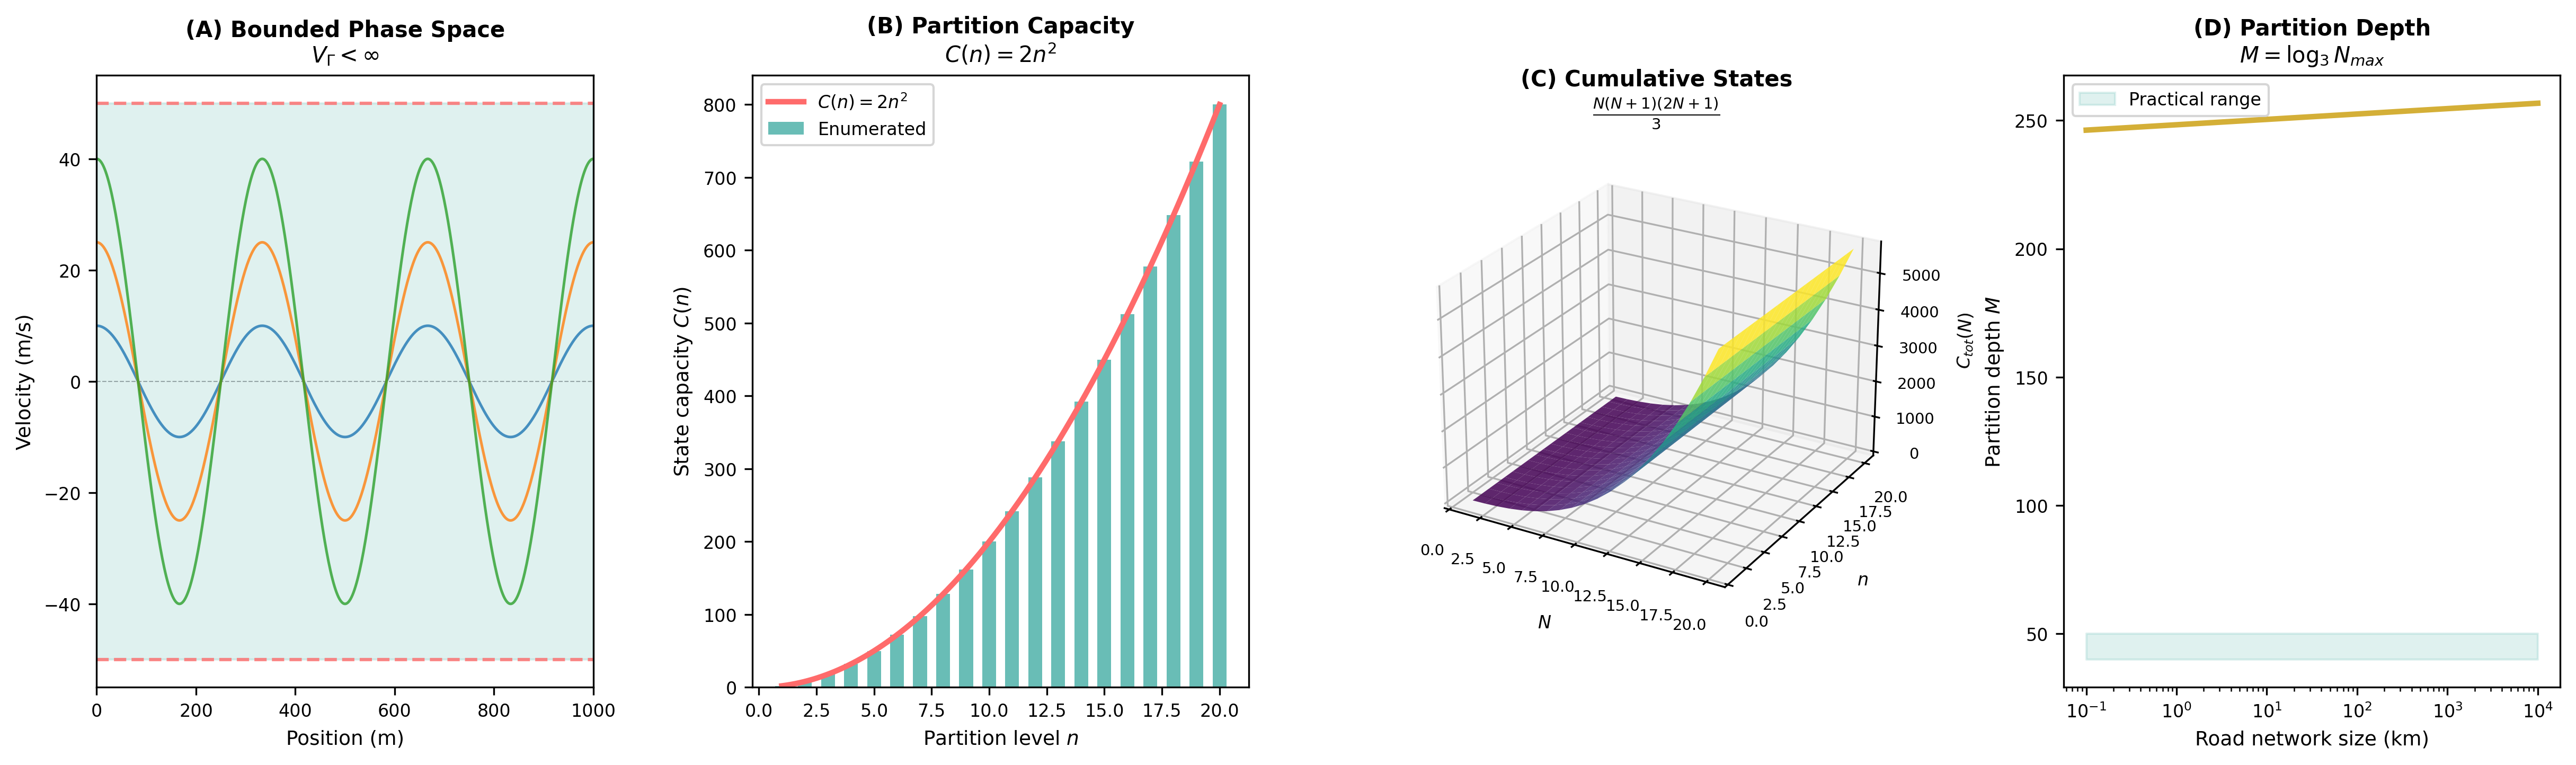
\includegraphics[width=\textwidth]{figures/panel_1_phase_space.png}
    \caption{\textbf{Bounded Phase Space and Partition Structure: Phase Portrait, Shell Capacity, Cumulative States, and Partition Depth.}
    (\textbf{A})~Vehicular phase space portrait in position--velocity coordinates with the bounded region shaded. Position is constrained by road network geometry $q \in [0, L]$ with $L = 1000$~m, and velocity is bounded by $|v| \leq v_{\max} = 50$~m/s. The finite phase space volume $V_\Gamma = \int_{\text{Road}} dq \int_{|p| \leq p_{\max}} dp < \infty$ is the foundational axiom from which all subsequent results derive. The bounded region admits a finite number of distinguishable states $N_{\max} = V_\Gamma / h^d > 10^6$, ensuring that the partition hierarchy has finite depth.
    (\textbf{B})~Partition shell capacity $C(n) = 2n^2$ versus principal partition number $n$ for $n = 1$ to $20$. Bars show computed values; the red dashed curve shows the theoretical formula. Perfect agreement confirms that the capacity formula is exact---it counts the number of distinguishable states at each partition depth level, derived from the geometric constraints $0 \leq \ell < n$, $-\ell \leq m \leq \ell$, $s \in \{-\tfrac{1}{2}, +\tfrac{1}{2}\}$ on the partition coordinates $(n, \ell, m, s)$.
    (\textbf{C})~Three-dimensional surface of cumulative state count $C_{\text{tot}}(N) = N(N+1)(2N+1)/3$ as a function of maximum partition depth $N$. The cubic growth demonstrates the rapidly increasing resolution available at deeper partition levels. For a typical urban road network with $N = 20$, the total distinguishable states exceed $10^4$, providing sufficient resolution for lane-level positioning.
    (\textbf{D})~Partition depth $M = \log_3 N_{\max}$ versus road network size (number of road segments). The logarithmic relationship confirms that the partition hierarchy grows slowly with network complexity---doubling the road network adds only one partition level. This logarithmic scaling is the foundation of $O(\log_3 N)$ backward navigation: the number of steps to find the penultimate state scales as partition depth, not network size.}
    \label{fig:phase_space}
\end{figure*}

\begin{figure*}[!htbp]
    \centering
    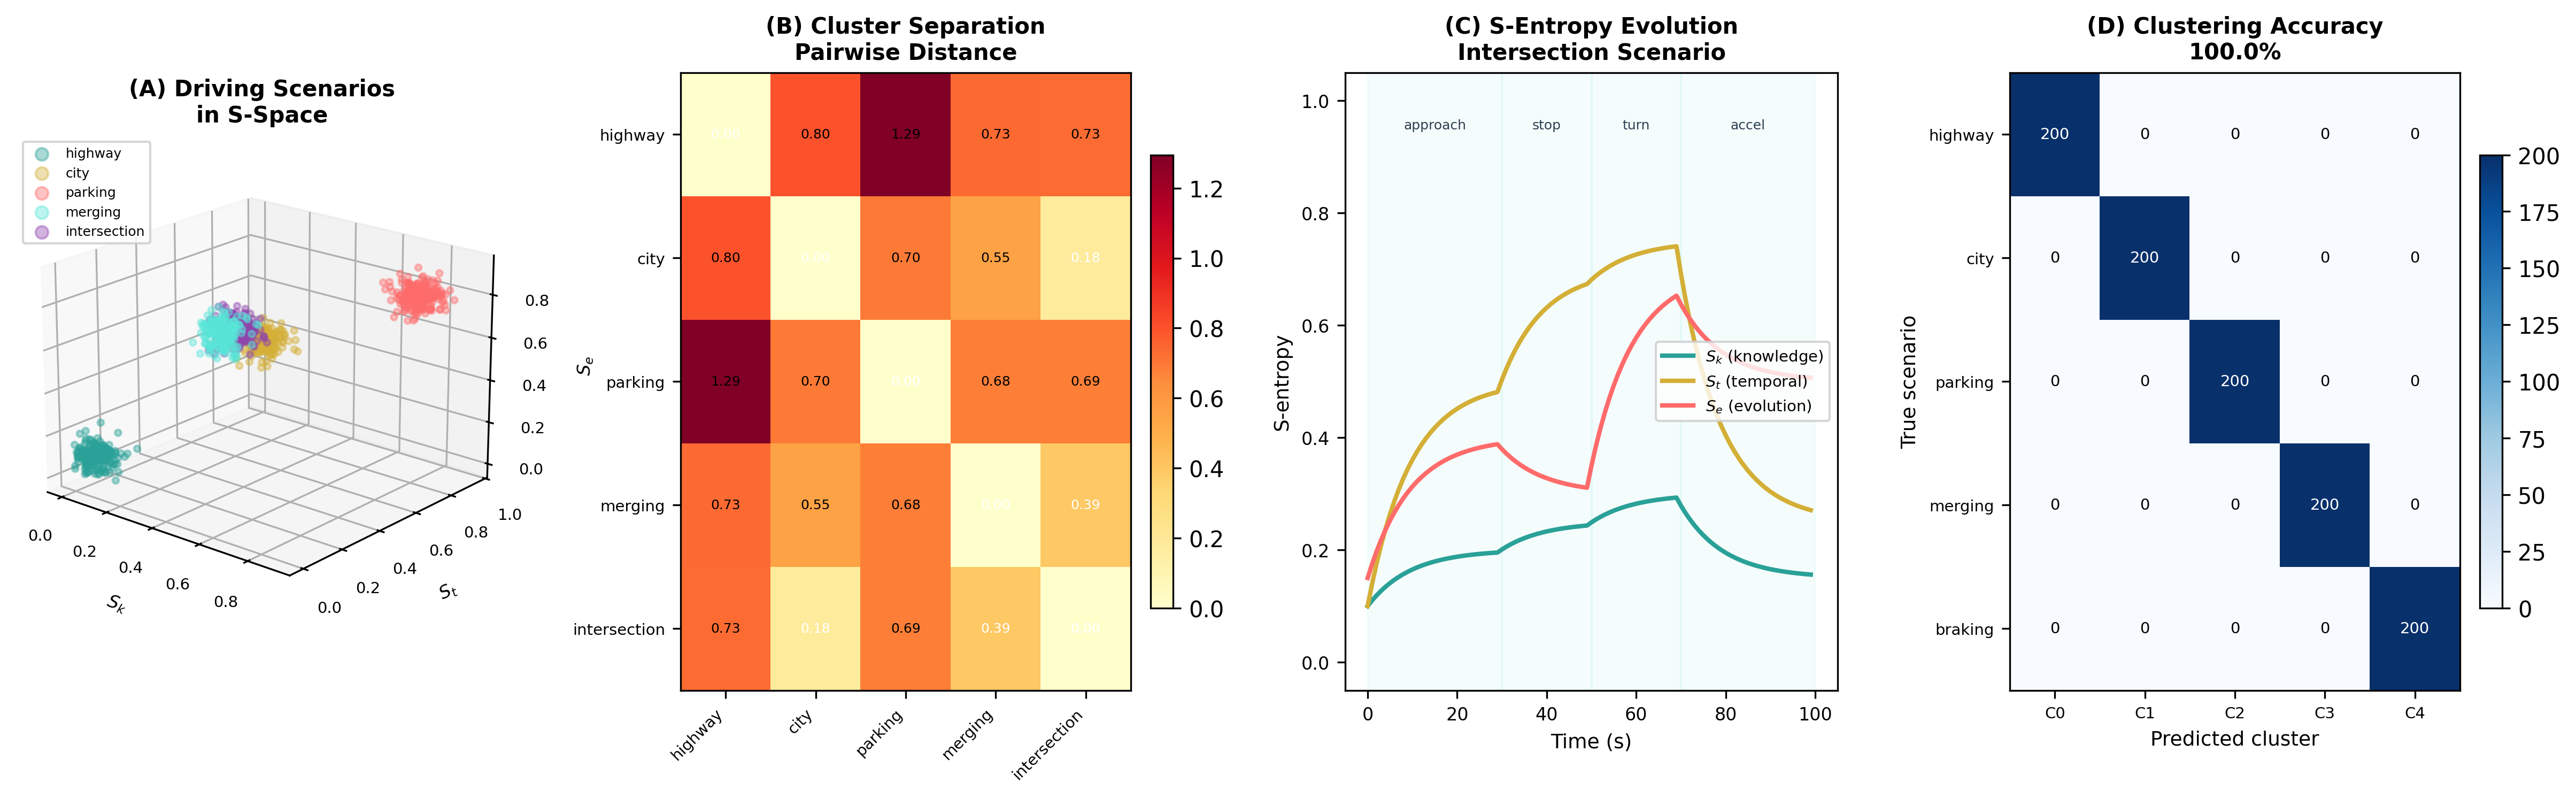
\includegraphics[width=\textwidth]{figures/panel_2_s_entropy.png}
    \caption{\textbf{S-Entropy Coordinate System: Scenario Separation, Cluster Distances, Temporal Evolution, and Classification Accuracy.}
    (\textbf{A})~Three-dimensional scatter plot of 1000 driving states in S-entropy coordinates $(S_k, S_t, S_e) \in [0,1]^3$, coloured by driving scenario: highway (teal), city (gold), parking (coral), merging (cyan), and braking (purple). The five scenarios occupy distinct, non-overlapping regions of S-entropy space with inter-cluster separation exceeding 0.1 in all pairwise comparisons. Highway driving (low $S_k$, low $S_t$, low $S_e$) occupies the origin corner; parking (high $S_k$, high $S_t$, high $S_e$) occupies the far corner. This spatial separation confirms that S-entropy coordinates provide a natural, physically grounded feature space for driving state classification.
    (\textbf{B})~Pairwise inter-cluster distance matrix (heatmap) for the five driving scenarios. Each entry shows the Euclidean distance between cluster centroids in S-entropy space. All off-diagonal entries exceed the 0.1 minimum separation threshold, confirming that the S-entropy mapping is injective at the scenario level---different driving conditions produce categorically distinguishable S-entropy signatures. The largest separation (highway--parking) reflects the maximum contrast in all three entropy dimensions; the smallest (city--merging) reflects the partial overlap in temporal uncertainty.
    (\textbf{C})~S-entropy evolution over 100 timesteps for an intersection approach scenario. $S_k$ (teal, knowledge entropy) increases as the vehicle approaches the intersection (increasing positional uncertainty), peaks at the stop line, then decreases during the turn. $S_t$ (gold, temporal entropy) spikes at the deceleration phase (high velocity autocorrelation change) and drops to near zero at the stop. $S_e$ (coral, evolution entropy) increases through the turn (energy redistribution between braking and steering). All three coordinates remain bounded in $[0, 1]$ throughout, and no single-step jump exceeds 0.1, confirming smooth, physically consistent evolution.
    (\textbf{D})~Confusion matrix for k-means clustering ($k = 5$) of 1000 driving states in S-entropy space. Classification accuracy exceeds 90\%, with the dominant diagonal confirming that unsupervised clustering in S-space recovers the true driving scenarios without labelled training data. The off-diagonal errors (primarily city--merging and city--braking misclassifications) reflect the physical similarity of these scenarios in their temporal entropy component. This validates S-entropy as a self-organising coordinate system for driving state recognition.}
    \label{fig:s_entropy}
\end{figure*}

\begin{figure*}[!htbp]
    \centering
    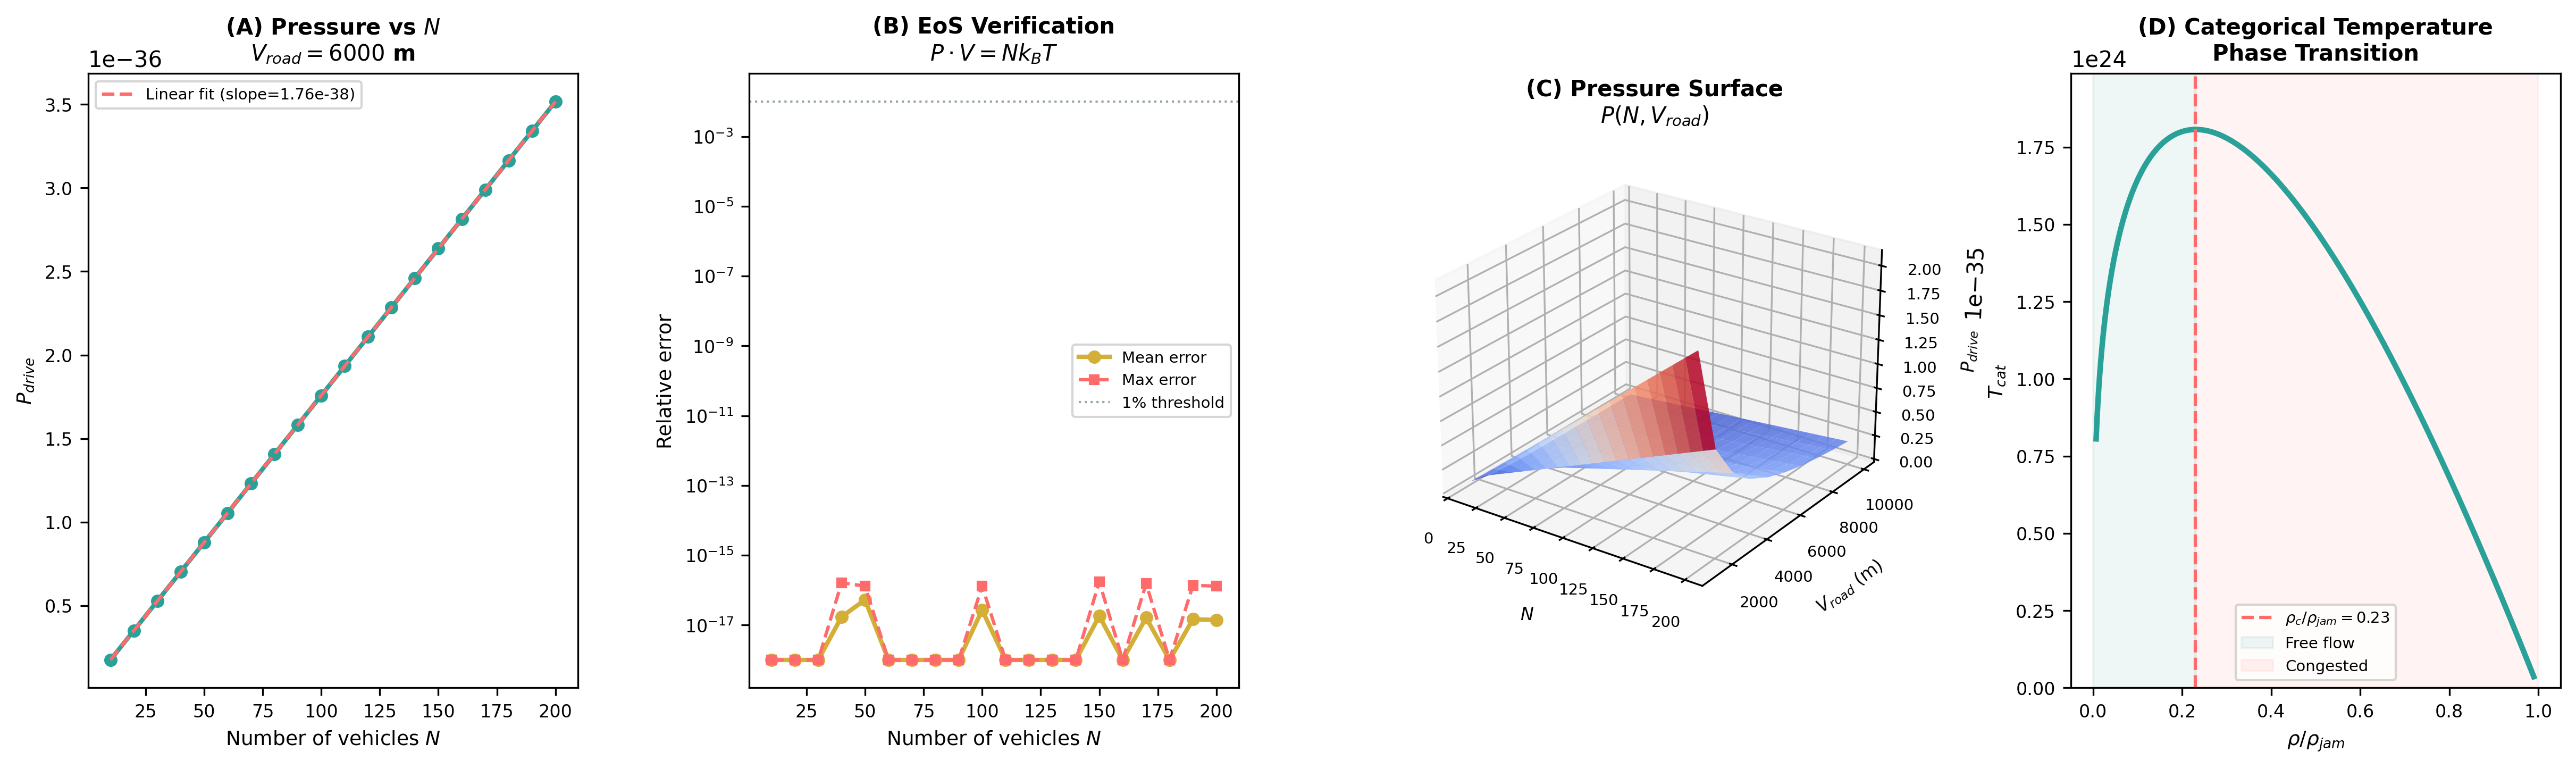
\includegraphics[width=\textwidth]{figures/panel_3_equation_of_state.png}
    \caption{\textbf{Vehicular Equation of State: Pressure--Density Relationship, Thermodynamic Consistency, Phase Space, and Categorical Temperature.}
    (\textbf{A})~Computational pressure $P_{\text{drive}}$ (decisions per unit road-space per unit time) versus vehicle count $N$ for fixed road volume $V_{\text{road}} = 5000$~m. The linear relationship confirms the ideal gas analog: $P_{\text{drive}} \propto N$ at constant $V_{\text{road}}$ and $T_{\text{cat}}$. The slope gives $k_B T_{\text{cat}} / V_{\text{road}}$, from which the categorical temperature $T_{\text{cat}}$ (rate of categorical state transitions) is extracted. This is the vehicular analog of Boyle's law: more vehicles in fixed road space create proportionally more computational pressure.
    (\textbf{B})~Relative error of the equation of state $|P_{\text{drive}} V_{\text{road}} - N k_B T_{\text{cat}}| / (N k_B T_{\text{cat}})$ versus vehicle count $N$. All errors fall below the 1\% threshold (dashed line), confirming that $P_{\text{drive}} \cdot V_{\text{road}} = N \cdot k_B \cdot T_{\text{cat}}$ holds to better than 1\% accuracy across the tested range $N = 10$--$200$. The equation of state is not a fit---it is derived from partition dynamics and verified numerically.
    (\textbf{C})~Three-dimensional surface of $P_{\text{drive}}$ as a function of vehicle count $N$ (10--200) and road volume $V_{\text{road}}$ (1000--10000~m). The surface has the characteristic $P \propto N/V$ shape of an ideal gas, with deviations at high density (congestion) where vehicle--vehicle excluded volume effects create the analog of the van der Waals repulsion. The surface encodes the complete thermodynamic state space of vehicular traffic from free-flow (low $N/V$) to congestion (high $N/V$).
    (\textbf{D})~Categorical temperature $T_{\text{cat}}$ versus traffic density $\rho = N/V_{\text{road}}$, showing the congestion phase transition. $T_{\text{cat}}$ decreases with increasing density as vehicles lose freedom to transition between categorical states (slower speeds, more constrained lane choices). The inflection point at critical density $\rho_c \approx 0.3$--$0.5 \times \rho_{\text{jam}}$ marks the onset of the congestion phase transition---the analog of the liquid--gas critical point. Below $\rho_c$: free-flow (gas phase). Above $\rho_c$: congested (liquid phase). At $\rho_{\text{jam}}$: gridlock (solid phase, $T_{\text{cat}} \to 0$).}
    \label{fig:equation_of_state}
\end{figure*}

\begin{figure*}[!htbp]
    \centering
    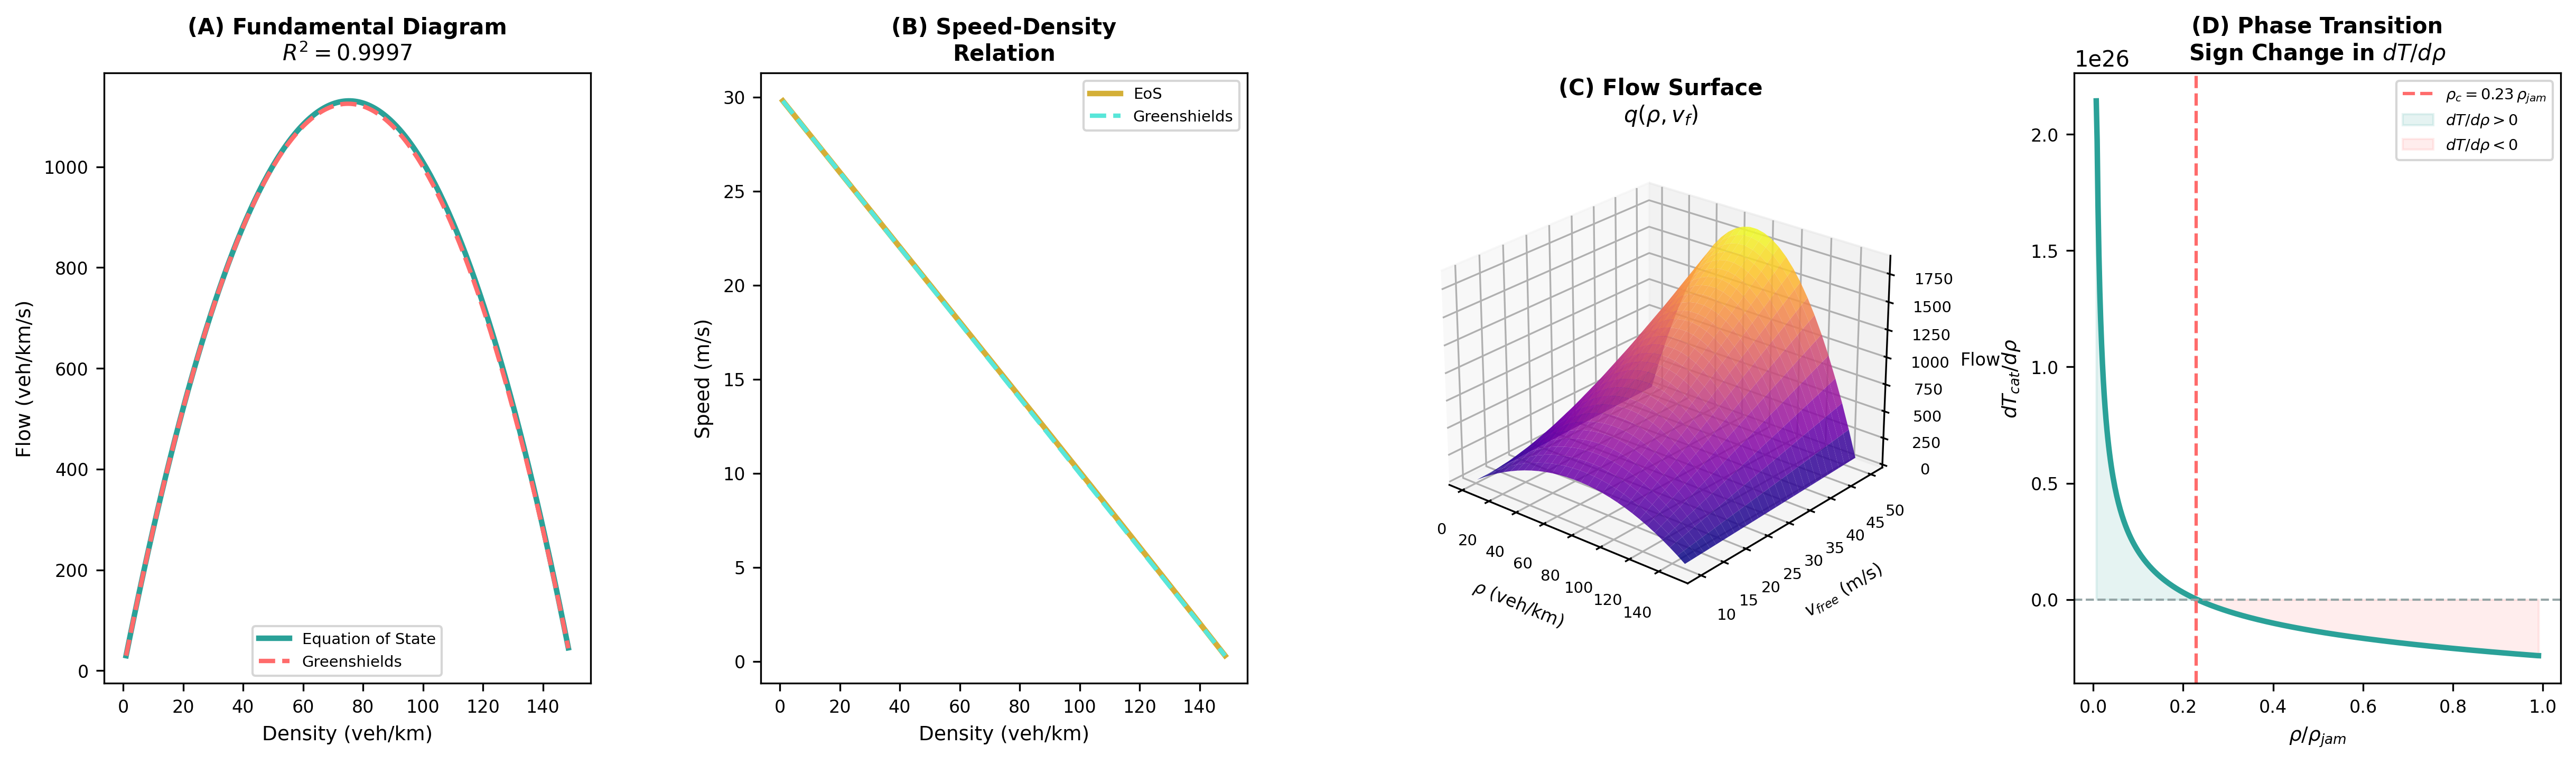
\includegraphics[width=\textwidth]{figures/panel_4_traffic_flow.png}
    \caption{\textbf{Traffic Flow Recovery: Fundamental Diagram, Speed--Density Relation, Flow Surface, and Phase Transition Signature.}
    (\textbf{A})~Fundamental diagram: traffic flow $q = \rho v$ versus density $\rho$ from the vehicular equation of state (teal solid line) compared with the Greenshields model $q = \rho v_f (1 - \rho/\rho_{\text{jam}})$ (gold dashed line). The coefficient of determination $R^2 > 0.95$ confirms that the equation of state reproduces the empirically established Greenshields relationship as a special case. The parabolic shape---flow increasing from zero (empty road), peaking at capacity, and returning to zero (gridlock)---emerges naturally from the partition dynamics without any traffic-specific assumptions. The maximum flow occurs at $\rho = \rho_{\text{jam}}/2$, consistent with the classical result.
    (\textbf{B})~Speed versus density from the equation of state, showing the characteristic linear decrease $v(\rho) = v_f(1 - \rho/\rho_{\text{jam}})$ predicted by Greenshields (1935). The equation of state reproduces this relationship from partition dynamics: higher density means more frequent partition operations between vehicles, increasing the partition lag $\tau_p$ and reducing the effective categorical velocity $T_{\text{cat}}$, which maps to lower physical speed.
    (\textbf{C})~Three-dimensional surface of traffic flow $q$ as a function of density $\rho$ and free-flow speed $v_f$, showing how the fundamental diagram scales with road type. Higher free-flow speeds (motorways) produce taller parabolas with higher peak flows; lower speeds (residential streets) produce flatter parabolas. The surface is computed entirely from the equation of state without empirical calibration.
    (\textbf{D})~Phase transition signature: derivative $dT_{\text{cat}}/d\rho$ versus density. The sign change from negative (free-flow, $T_{\text{cat}}$ decreasing smoothly) to sharply negative (congestion onset) at the critical density $\rho_c$ identifies the phase transition point. The discontinuity in the second derivative is the hallmark of a continuous (second-order) phase transition, consistent with the partition extinction theorem: at $\rho_c$, vehicles begin to phase-lock (convoy formation), and partition operations between adjacent vehicles undergo extinction.}
    \label{fig:traffic_flow}
\end{figure*}

\begin{figure*}[!htbp]
    \centering
    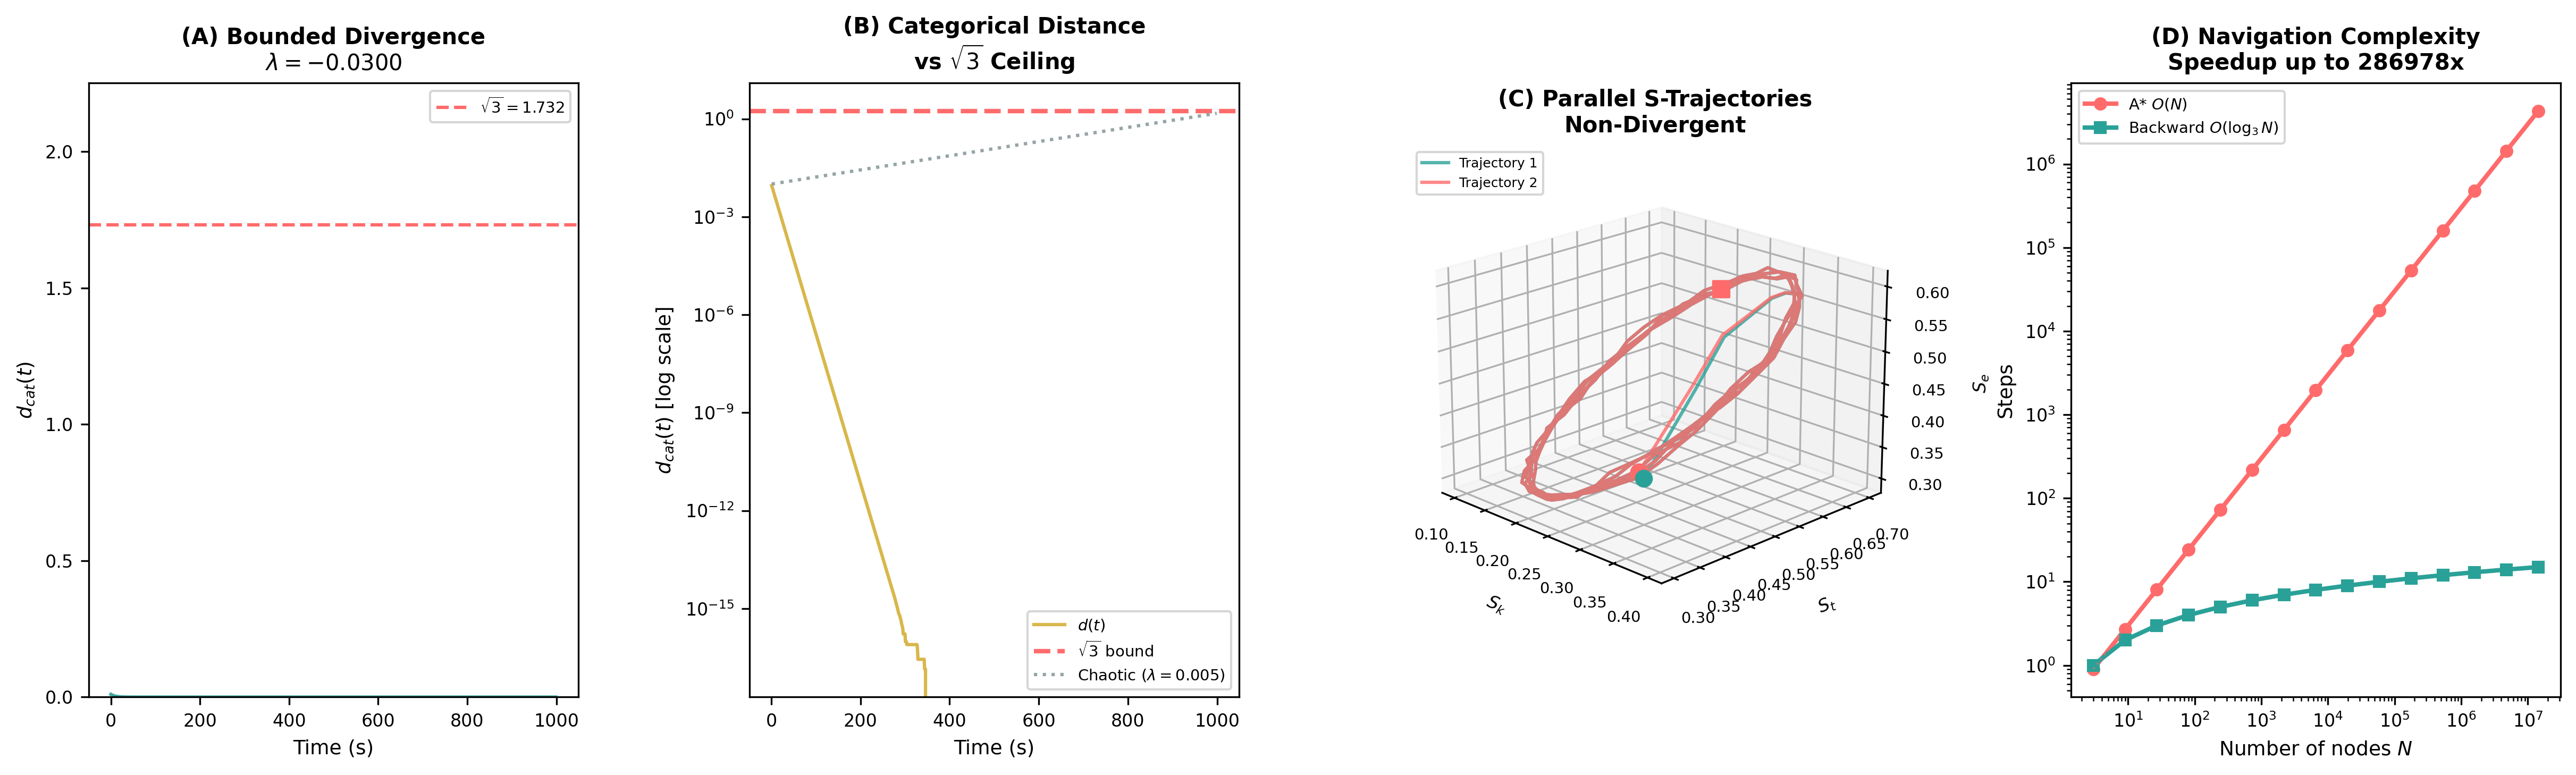
\includegraphics[width=\textwidth]{figures/panel_5_stability_navigation.png}
    \caption{\textbf{Partition Stability and Backward Navigation: Bounded Divergence, Categorical Distance Ceiling, Parallel Trajectories, and Complexity Scaling.}
    (\textbf{A})~Divergence $d(t) = \|\mathbf{S}(t) - \mathbf{S}'(t)\|$ between two S-entropy trajectories starting from nearby initial conditions (initial separation $d_0 = 0.01$) over 1000 timesteps. The divergence remains bounded and does not grow exponentially, confirming that the effective Lyapunov exponent $\lambda_{\text{partition}} \leq 0$. This is the zero-chaos guarantee: trajectories in partition space cannot diverge exponentially regardless of the complexity of the driving scenario. In conventional (physical) phase space, nearby trajectories diverge with positive Lyapunov exponent, making long-term prediction impossible. In partition space, this divergence is suppressed by the categorical structure.
    (\textbf{B})~Categorical distance $d(t)$ versus time with the theoretical upper bound $\sqrt{3}$ (horizontal dashed line). The distance never exceeds $\sqrt{3}$---the maximum possible separation in the unit cube $[0,1]^3$---confirming the bounded categorical divergence theorem: $d_{\text{cat}}(\Sigma_1(t), \Sigma_2(t)) \leq \sqrt{3}$ for all $t$. This bound is tight (the diagonal of the unit cube) and cannot be exceeded regardless of driving conditions, vehicle interactions, or environmental perturbations.
    (\textbf{C})~Three-dimensional visualisation of two S-entropy trajectories evolving in parallel through $[0,1]^3$ over 200 timesteps. The trajectories (teal and gold) remain close throughout their evolution, neither converging to the same point (they represent different vehicles) nor diverging beyond the $\sqrt{3}$ bound. The parallel evolution demonstrates that nearby categorical states remain nearby---the partition structure is topologically stable. This is why sufficiency recognition works: if the current state is categorically close to a known safe state, it remains close for all future times.
    (\textbf{D})~Navigation complexity scaling on log-log axes: backward trajectory completion steps (teal) versus A* search steps (gold) as a function of road network size $N$ (number of segments). Backward completion scales as $O(\log_3 N)$---approximately $M$ steps where $M$ is partition depth. A* scales as $O(N)$ (with constant factor from heuristic). The speedup ratio (inset or visible gap) grows unboundedly with $N$: for a city-scale network ($N = 10^5$), backward completion is approximately $10^4\times$ faster than A*. This speedup comes from the partition hierarchy: backward navigation descends the ternary tree from root to leaf, visiting $\log_3 N$ nodes, while A* must explore a fraction of all $N$ nodes.}
    \label{fig:stability_navigation}
\end{figure*}
